%\documentclass[12pt]{aastex}
\documentclass[iop]{emulateapj}
%\documentclass{article}
%\usepackage{draftwatermark}
\usepackage{paralist}
\shorttitle{Vertical shear instability}
\shortauthors{M-K. Lin, A. Youdin}

\usepackage{amsmath}
%\usepackage{url}
\usepackage{bm}
%\usepackage[font=small,format=plain,labelfont=bf,up,textfont=it,up]{caption}
\newcommand{\p}{\partial}
\newcommand{\lmax}{l_\mathrm{max}}
\newcommand{\sbar}{\bar{\sigma}} 
\newcommand{\He}{\operatorname{He}}
\newcommand{\imgi}{\mathrm{i}} 
\newcommand{\ii}{\mathrm{i}}
\newcommand{\C}{\mathcal{C}^\lambda}
\newcommand{\wop}[1]{\mathcal{V}^{(#1)}}
\newcommand{\avg}[1]{\langle{#1}\rangle}
%\newcommand{\max}[1]{\mathrm{max}({#1})}
%\newcommand{\min}[1]{\mathrm{min}({#1})}
\newcommand{\zhat}{\hat{z}}
\newcommand{\rhat}{\hat{r}}
\newcommand{\he}{\mathcal{H}}
\newcommand{\amp}{\mathcal{A}}
\newcommand{\dd}{\delta}
\newcommand{\real}{\operatorname{Re}}
\newcommand{\imag}{\operatorname{Im}}
\newcommand{\sgn}{\operatorname{sgn}}
\newcommand{\zmax}{Z_s}
\newcommand{\wbar}{\tilde{W}}
\newcommand{\qbar}{\tilde{Q}}
\newcommand{\dbigH}{\frac{H^\prime}{H}}
\newcommand{\Rp}{\frac{\rho_0^\prime}{\rho_0}}
\newcommand{\Fp}{\frac{g^\prime}{g}}
\newcommand{\Rpp}{\frac{\rho_0^{\prime\prime}}{\rho_0}}
\newcommand{\Fpp}{\frac{g^{\prime\prime}}{g}}
\newcommand{\ils}{L_s^{-1}}
\newcommand{\ilp}{L_p^{-1}}
\newcommand{\ihp}{H_p^{-1}}
\newcommand{\ihs}{H_s^{-1}}
\newcommand{\ciso}{c_\mathrm{iso}}
\newcommand{\csmid}{c_{s0}} 
\newcommand{\hiso}{h_\mathrm{iso}}
\newcommand{\Hiso}{H_\mathrm{iso}}
\newcommand{\zeus}{\texttt{ZEUS-MP }}
\newcommand{\rsph}{r_\mathrm{sph}}
\newcommand{\dvx}{\dd v_x}
\newcommand{\dvy}{\dd v_y}
\newcommand{\dvz}{\dd v_z}
\newcommand{\dbx}{\dd B_x}
\newcommand{\dby}{\dd B_y}
\newcommand{\dbz}{\dd B_z}
\newcommand{\w}{ \widetilde{W}}
%\newcommand{\sbar}{\bar{\sigma}}
\newcommand{\dphi}{\dd \Phi}
\newcommand{\actaa}{Acta Astron.}
\defcitealias{lin12}{L12} 

\begin{document}

\title{Linear vertical shear instability in astrophysical disks: a parameter study}

\author{Min-Kai Lin, Andrew Youdin}
\affil{ $^1$Department of Astronomy and Steward Observatory, University of
  Arizona, 933 North Cherry Avenue, Tucson, AZ 85721, USA}
\email{minkailin@email.arizona.edu}

\begin{abstract}
  
\end{abstract}

\section{Introduction}

\section{Governing equations and disk models}\label{setup}
We consider  an inviscid, non-self-gravitating three-dimensional (3D)
disk orbiting a central star of mass $M_*$. We adopt cylindrical
co-ordinates $(r,\phi, z)$ centered on the star to describe the global
disk. The governing fluid equations are
\begin{align}
  &\frac{\p\rho}{\p t} + \nabla\cdot{\left(\rho\bm{v}\right)} = 0,\\
  &\frac{\p\bm{v}}{\p t} + \bm{v}\cdot\nabla\bm{v} =
  -\frac{1}{\rho}\nabla P - \nabla\Phi_*,\\
  &\frac{\p P}{\p t} + \bm{v}\cdot\nabla P  = - \gamma P
  \nabla\cdot\bm{v} - \Lambda % \frac{\rho}{t_c}\left(\frac{P}{\rho} -
    % \left.\frac{P}{\rho}\right|_{t=0}\right)
  , \label{full_energy}
\end{align}
where $\rho$ is the mass density, $\bm{v}$ is the velocity field (the
rotation frequency being $\Omega=v_\phi/r$), $P$
is the pressure, $\gamma$ is the constant adiabatic index, and $\Phi_*
= -GM_*(r^2 + z^2)^{-1/2}$ is the gravitational potential of the
central star and $G$ is the gravitational constant. 
In the energy equation (Eq. \ref{full_energy}) the source term
$\Lambda$ represent non-adiabatic effects which we
model below. The gas temperature $T$ is defined through the ideal gas 
equation of state,  
\begin{align}
P = \frac{\mathcal{R}}{\mu}\rho T,
\end{align}
where $\mathcal{R}$ is the gas constant and $\mu$ is the mean molecular
weight.    

\subsection{Thermal relaxation}
We model non-adiabatic effects by defining $\Lambda$ as a thermal
relaxation term,
\begin{align}\label{thermal_relax}
  \Lambda  \equiv \frac{\rho\mathcal{R}}{\mu t_c}\left(T - T_0\right),
\end{align}
where $T_0=T_0(r,z)$ is the initial temperature, and $t_c$ is a
thermal relaxation timescale parametrized via $\beta$ such that 
\begin{align}\label{beta_def}
  t_c = \beta \Omega_k^{-1},
\end{align}
where $\Omega_k=\sqrt{GM_*/r^3}$ is the Keplerian frequency.   

For most of this paper we will take $\beta$ as a constant input
parameter, so that we can vary the thermodynamic response of the
disk from isothermal ($\beta\ll 1$) to adiabatic ($\beta \gg 1$) in a
controlled manner. However, for application to protoplanetary disks in 
\S\ref{application} we will model $\beta$ based on physical thermal
timescales, in which case $\beta$ is determined by the equilibrium
disk properties and the perturbation lengthscales of interest.  

\subsection{Baroclinic disk equilibria}\label{eqm}
The equilibrium disk is steady and axisymmetric with density,
pressure and rotation profiles $\rho(r,z)$, $P(r,z)$ and
$\Omega(r,z)$, respectively. These functions satisfy  
\begin{align}
  0 &= \frac{1}{\rho}\frac{\p P}{\p z} + \frac{\p \Phi_*}{\p z},\label{vert_equilibrium}\\
  r\Omega^2&= \frac{1}{\rho}\frac{\p P}{\p r} + \frac{\p \Phi_*}{\p
    r}.\label{hori_equilibrium} 
\end{align} 
These equations allows us to choose any mid-plane density 
distribution $\rho_0(r)\equiv \rho(r,0)$. In this work we assume a
power-law profile, 
\begin{align}
  \rho_0(r) = \rho_{00}\left(\frac{r}{r_0}\right)^p,
\end{align}
where $\rho_{00}$ is the midplane density at the fiducial radius
$r=r_0$ and $p$ is the power-law index.  

We consider disk equilibria in which the pressure $P$ and density
$\rho$ are related by   
\begin{align}
  P(r,z) &= 
  \frac{c_{s0}^2(r)}{\Gamma}\rho_0(r)^{1-\Gamma}\rho^\Gamma(r,z),\notag\\
  & \equiv K(r)\rho^{\Gamma}(r,z). \label{eqm_press}
\end{align}
where the polytropic index $\Gamma$ is a  constant parameter  and the
function $c_{s0}(r)$ is prescribed below. Choosing $\Gamma=1$ gives 
locally vertically isothermal disk and $c_{s0}(r)$ is the mid-plane
sound-speed. %For $\Gamma=\gamma$ the disk is adiabatically stratified
% in the vertical 
It shall be convenient to define the function $c_s(r,z)$ 
\begin{align}
  c_s^2\equiv % \frac{dP}{d\rho} =
  c_{s0}^2(r)\left(\frac{\rho}{\rho_0}\right)^{\Gamma-1} =
  \frac{\Gamma P}{\rho}, 
\end{align}
which is related to the isothermal sound-speed $c_\mathrm{iso} =
c_s/\sqrt{\Gamma}$. We take $c_{s0}(r)$ to be another power-law:  
\begin{align}
  c_{s0}^2(r)=c_{s00}^2\left(\frac{r}{r_0}\right)^q, 
\end{align}
where $c_{s00}\equiv c_{s0}(r_0)$  and $q$ is the power-law index, and
define   
\begin{align}
  \epsilon(r) \equiv \frac{c_{s0}(r)}{v_k(r)} \equiv
  \frac{H}{r} 
\end{align}
to parametrize the magnitude of the sound-speed, where
$v_k=r\Omega_k$ is the Keplerian azimuthal velocity and
$H$ is a characteristic scale-height.  Thus, $\epsilon$
is also a characteristic disk aspect-ratio.  In practice, we consider
thin disks with $\epsilon \ll 1$. 

For discussion purposes it is useful to define the vertical buoyancy
frequency $N_z$ via
\begin{align}
  N_z^2 \equiv - c_p^{-1}g_z \frac{\p S}{\p z} = c_s^2 \left(\frac{\gamma -
      \Gamma}{\gamma}\right)\left(\frac{\p\ln\rho}{\p z}\right)^2,   
\end{align}
where $c_p$ is the heat capacity at constant pressure, $g_z\equiv
\rho^{-1}\p_zP $ and $S\equiv c_p\ln{P^{1/\gamma}/\rho}$ is the
specific entropy. The second equality applies to the disk equilibria
described above. 
We are interested in
neutrally or sub-adiabatically stratified 
disks with $\Gamma\leq \gamma$ so that $N_z^2\geq0$.  

%\subsection{Vertical structure}

Solving the equilibrium disk equations, we find the explicit
expression for the density field for 
$\Gamma\neq1$ is given  by
\begin{align}\label{eqm_dens}
  &\left(\frac{\rho}{\rho_0}\right)^{\Gamma-1} = 1 +
  \frac{\left(\Gamma-1\right)}{\epsilon^2}\left(\frac{1}{\sqrt{1+z^2/r^2}}-1\right).
\end{align}
Note that for $\Gamma > 1 + \epsilon^2$ there is a disk surface $H_s$
such that $\rho(r,H_s)=0$. 
% Note that for $\Gamma\neq1$ the disk has a surface $z=H(r)$ such that
% $\rho(r,H)=0$. If we parametrize
% \begin{align}
%   H(r)\equiv h r,
% \end{align}
% then the imposed sound-speed and disk thickness are related by 
% \begin{align}
%   h^2(r) = \left[1-\frac{\epsilon^2(r)}{\Gamma-1}\right]^{-2}-1. 
% \end{align}

Similarly, the equilibrium rotation is 
\begin{align}\label{eqm_rot}
  \frac{\Omega^2(r,z)}{\Omega_k^2(r)}=1 +
  \left(p+\frac{s}{\Gamma}\right)\epsilon^2(r) 
  +\frac{s}{\Gamma} \left(1-\frac{1}{\sqrt{1+z^2/r^2}}\right), 
\end{align}
where $s\equiv q+p(1-\Gamma)$. We also define % the radial shear rate  
% \begin{align}
%   S(r,z) \equiv r\frac{\p\Omega}{\p r},  
% \end{align}
% and
the square of the epicyclic frequency $\kappa$ 
\begin{align}
  \kappa^2(r,z) \equiv \frac{1}{r^3}\frac{\p }{\p
    r}\left(r^4\Omega^2\right). %2\Omega(2\Omega + S). 
\end{align}


\subsubsection{Vertically isothermal disks}
For $\Gamma=1$ the equilibrium density $\rho(r,z)$ and rotation
$\Omega(r,z)$ are given by 
\begin{align}
  \frac{\rho(r,z)}{\rho_0(r)} &=
  \exp{\left[\frac{1}{\epsilon^2}\left(\frac{1}{\sqrt{1+z^2/r^2}}-1\right)\right]}\\    
  \frac{\Omega^2(r,z)}{\Omega_k^2(r)}& =1+ (p+q)\epsilon^2(r) + q\left(1 -
    \frac{1}{\sqrt{1+z^2/r^2}}\right),\label{vertiso_eqm}
\end{align}
which may be obtained from Eq. \ref{eqm_dens} and Eq. \ref{eqm_rot} by
taking the limit $\Gamma\to 1$. We will, in fact, primarily focus on
vertically isothermal disks which is the relevant case for irradiated
protoplanetary disks \citep{chiang97}. 


\subsection{Vertical shear}\label{vshear_def}
Note that the disk is in general baroclinic with $\Omega =
\Omega(r,z)$. This is explicit from Eq. \ref{eqm_rot} and Eq. \ref{vertiso_eqm}, but is also 
implied by Eq. \ref{vert_equilibrium}---\ref{hori_equilibrium} and 
Eq. \ref{eqm_press},  
\begin{align}
  r\frac{\p\Omega^2}{\p z} = - \rho^{\Gamma-1}\frac{\p\ln\rho}{\p
    z}\frac{dK}{dr} = - \frac{g_z}{\Gamma}\frac{d\ln K}{dr}.\label{vertical_shear}
\end{align}
Evaluating this expression explicitly,
\begin{align}
  r\frac{\p\Omega^2}{\p z} = \frac{sz\Omega_k^2}{\Gamma
    r\left(1+z^2/r^2\right)^{3/2}}. \label{vertical_shear_ex} 
\end{align}
Note that there is a maximum vertical shear rate at $z=r/\sqrt{2}$,
which is expected to limit the growth rate of unstable modes.    


\subsection{Stability condition against axisymmetric adiabatic
  perturbations}\label{solberg}
A rotating flow is stable against axisymmetric adiabatic perturbations
if both Solberg-Hoiland criteria  are satisfied:
\begin{align}
  \kappa^2 - \frac{1}{\rho c_p}\nabla P \cdot \nabla S &> 0,\\
  -\frac{\p P}{\p z}\left(\frac{\p j^2}{\p r}\frac{\p S}{ \p z} -
    \frac{\p j^2}{\p z}\frac{\p S}{\p r} \right)&>0. \label{second_SH} 
\end{align}
\citep{tassoul78}, where $j=r^2\Omega$ is the specific angular
momentum. For rotationally-supported, thin disks, pressure gradients are small 
compared to rotation, so the first criterion is generally
satisfied. Thus, to assess stability, we consider the second
criterion. For our disk models,
\begin{align}
  &\frac{\p S}{\p r} = c_p\left[\frac{s}{\gamma r} +
    \left(\frac{\Gamma}{\gamma}-1\right)\frac{\p \ln{\rho}}{\p
       r}\right],\\
  &\frac{\p S}{\p z} = c_p
  \left(\frac{\Gamma}{\gamma}-1\right)\frac{\p \ln{\rho}}{\p z}. 
\end{align} 
Without loss of generality, we evaluate Eq. \ref{second_SH} in $z>0$
where $\p_zP<0$. Here we approximate $\p_r j^2\simeq r^3\Omega_k^2$ but
use Eq. \ref{vertical_shear} for $\p_zj^2$. Then 
\begin{align}\label{solberg2}
  % \gamma - \Gamma > \frac{s\epsilon^2}{\Gamma}
  % \left(\frac{\rho}{\rho_0}\right)^{\Gamma-1} \left[s
  %   -\left(\gamma-\Gamma\right)\frac{\p\ln{\rho}}{\p\ln{r}} \right]. 
  \gamma - \Gamma > \frac{\epsilon^2}{\Gamma}
  \left(\frac{\rho}{\rho_0}\right)^{\Gamma-1} \left[s^2
    -s\left(\gamma-\Gamma\right)\frac{\p\ln{\rho}}{\p\ln{r}} \right]
\end{align} 
implies stability. For typical model parameters the right hand
side (RHS) is $O(\epsilon^2)$. Hence, instability in the adiabatic limit  
requires $\gamma < \Gamma + O(\epsilon^2)$. Since we consider
$\epsilon\ll1$, this implies the equilibrium disk must have a small
entropy gradient in order to be unstable to axisymmetric adiabatic
perturbations. This is generally not true for irradiated, stably
stratified disks \citep{chiang97}, in which the VSI requires rapid
thermal relaxation, as shown below. 

\section{Linear problem}\label{linear}
We consider axisymmetric perturbations to the above equilibria in the
form 
\begin{align}
  \rho \to \rho(r, z) + \delta\rho(r,z)\exp{\left( - \ii\sigma
      t\right)},    
\end{align}
and similarly for other fluid variables, where $\sigma = \omega + \ii
\nu$ is a (generally) complex frequency, with $\omega$ and $\nu$ being
the real frequency and growth rate, respectively.

The linearized fluid equations in cylindrical co-ordinates are  
\begin{align}
  \ii\sigma\delta\rho &= \frac{\rho}{r}\frac{\p}{\p r}\left(r\delta v_r\right) + \frac{\p}{\p
    z}\left(\rho\delta v_z\right)  + \hat{g}_c\frac{\p\rho}{\p r}\delta v_r,\\
  \ii\sigma\delta v_r &= \frac{1}{\rho}\frac{\p\delta P}{\p r} - 2\Omega
  \delta v_\phi - \hat{g}_c\frac{\delta\rho}{\rho^2}\frac{\p P}{\p r},\\ 
  \ii\sigma\delta v_\phi  &= \frac{\kappa^2}{2\Omega}\delta v_r +
  r\frac{\p\Omega}{\p z}\delta v_z,\\
  \ii \sigma\delta v_z &= \frac{1}{\rho}\frac{\p\delta P}{\p z} -
  \frac{\delta \rho}{\rho^2}\frac{\p P}{\p z},\\
  \ii\sigma\delta P &=\frac{\p P}{\p z}\delta v_z + \gamma P
  \left[\frac{1}{r}\frac{\p}{\p r}\left(r\delta v_r\right) + \frac{\p
      \delta v_z}{\p z}\right]\notag \\
  &+ \frac{1}{t_c}\left(\delta P -  
    \frac{P}{\rho}\delta\rho\right) + \hat{g}_c \frac{\p P}{\p r}\delta v_r,\label{full_energy1}
\end{align}
where the coefficients $\hat{g}_c=1$ are inserted to label terms
associated with the background radial disk structure. 

\subsection{Radially-local approximation}  
We consider perturbations with small radial lengthscales 
so that we can ignore the radial variations in the background
structure and radial gradients. We thus evaluate all coefficients in
the above equations at the fiducial radius $r=r_0$. However, the full
vertical dependence of the coefficients are retained. Then we can
assume perturbations have spatial dependence in the form
\begin{align}
  \delta \rho(r,z) \to \delta\rho(z)\exp{\ii k_r r}.
\end{align}
We take $k_r>0$ without loss of generality, and further assume $k_rr\gg1$ so that curvature terms can also be 
ignored.       

In order to emphasize the radially-local approximation, we
introduce the local Cartesian co-ordinates $(x,y,z)$ corresponding to
the the local $(r,\phi,z)$ directions, respectively. Then writing
$\delta P /\rho \equiv W$ and $c_s^2\delta\rho/\rho\equiv Q$, the
linearized system of equations are 
\begin{align}
  \ii\sigma \frac{Q}{c_s^2}  &=  \ii k_x \delta v_x + \frac{d\dd
    v_z}{dz} + \frac{\p\ln{\rho}}{\p z}\delta v_z + \hat{g}_c
  \frac{\p\ln{\rho}}{\p r} \delta v_x,\label{lin_mass}\\
  \ii\sigma \delta v_x  &= \ii k_x W - 2\Omega\delta v_y -
  \hat{g}_c\frac{1}{\rho}\frac{\p P}{\p r}\frac{Q}{c_s^2}\label{lin_vx}\\
   \ii \sigma\delta v_y &= r\frac{\p \Omega}{\p z}\delta v_z +
  \frac{\kappa^2}{2\Omega}\delta v_x, \label{lin_vy}\\
   \ii\sigma\delta v_z &= \frac{dW}{dz} +
  \frac{\p\ln{\rho}}{\p z}\left(W-Q\right), \label{lin_vz}\\
  \ii \sigma W &= c_s^2\frac{\p\ln{\rho}}{\p z}\delta v_z +
  c_s^2\frac{\gamma}{\Gamma} \left(\ii k_x\delta v_x + \frac{d\delta
      v_z}{dz}\right) \notag\\
  &+ \frac{1}{t_c}\left(W - \frac{Q}{\Gamma}\right) +
  \hat{g}_c\frac{1}{\rho}\frac{\p P}{\p r}\delta v_x,\label{lin_energy}
  % -&\ii\sigma W + \frac{1}{t_c}\left(W-\frac{Q}{\Gamma}\right) = -\ii\sigma\frac{\gamma}{\Gamma} Q +
  % c_s^2\frac{d\ln{\rho}}{dz}\left(\frac{\gamma}{\Gamma}-1\right)\delta v_z.\label{lin_energy}
\end{align}
where we have made the notation change $k_r\to k_x$. 
It is understood that the quantities $\rho,\,c_s^2,\,\Omega,\kappa,\, 
\p_z\Omega,\, \p_r\ln{\rho} $ and $ \p_r P$ are evaluated at $r=r_0$
using their expressions in the global disk given in \S\ref{setup}. 
Eq. \ref{lin_mass}---\ref{lin_energy} will form the basis of our numerical
study, but for analytical discussion
we will make further simplifications. 


% The radially-local approximation above is similar in spirit to the
% shearing box framework \citep{goldreich65} or the generalization
% thereof \citep{mcnally14}. The main difference being the terms
% proportional to $\hat{g}_c$ are neglected in the shearing box. 

\section{Vertical shear instability of locally
  isothermal perturbations}
{\bf need to update notation, use $\epsilon$ instead of $h$}
The linear problem simplifies considerably for the case
$\Gamma=\gamma=1$. Then 
\begin{align}
  W=Q. 
\end{align}
%so that
%\begin{align}
 % \delta v_z = \frac{1}{\ii\sigma}\frac{dQ}{dz}. 
%\end{align}
%Inserting this into the expression for $\delta v_x$ and the continuity
%equation, 
Inserting this into Eq. \ref{ode_w} gives a single equation for the linear stability
problem for isothermal perturbations in a vertically isothermal disk, 
\begin{align}\label{iso_ode}
  \frac{d^2Q}{dz^2} + \left(\frac{d\ln{\rho}}{dz} - \frac{\ii k_x
      r}{D}\frac{d\Omega^2}{dz}\right) \frac{dQ}{dz} +
  \sigma^2\left(\frac{1}{c_s^2} + \frac{k_x^2}{D}\right)Q=0, 
\end{align} 
subject to appropriate boundary conditions. 

We remark that Eq .\ref{iso_ode} is also applicable for
$\gamma=\Gamma\neq 1$ in the limit $t_c\to\infty$, since in that case
$W\simeq Q$ as well. The following discussion therefore also holds for
vertically non-isothermal, adiabatic disks.   

\subsection{Approximations}
Eq. \ref{iso_ode} is still complicated because the coefficients depend
on $z$ in a non-trivial manner. Furthermore, the eigenfrequency
$\sigma^2$ appears in $D$. In order to make progress, in this section
we make the following approximations. 

\emph{Thin disk.} We consider thin disks with $h\ll1$, so we may expand the
background density and vertical shear in powers of $z/r$. To lowest
order we obtain
\begin{align}
  &\rho(z) \simeq \rho_{00} \exp{\left(-\frac{z^2}{2H^2}\right)},\\
  &\frac{d\Omega^2}{dz} \simeq \frac{q\Omega_k^2z}{r^2}. 
\end{align}

\emph{Low frequency.} We consider eigenvalues such that
$|\sigma^2|\ll \kappa^2$. Then we can replace $D=\kappa^2 -\sigma^2\to
\kappa^2$. The problem simplifies because the eigenvalue now only
appears in the last term in Eq. \ref{iso_ode}. 

% \emph{Nearly constant $\kappa$}. We are mainly interested in the
% effect of vertical shear, i.e. $q\neq 0$. This is already captured
% explicitly in Eq. \ref{iso_ode}. We therefore simplify further by
% ignoring the vertical dependence of $\kappa^2$. In a thin disk, this
% quantity is nearly Keplerian.

With the above approximations and introducing the dimensionless
vertical co-ordinate $\hat{z} \equiv z/H$, the governing equation becomes
\begin{align}\label{iso_ode2}
  &\frac{d^2Q}{d\hat{z}^2} - \left[ 1 + \ii qh
    \left(k_xH\right)\frac{\Omega_k^2}{\kappa^2}\right]\hat{z}\frac{dQ}{d\hat{z}}\notag\\
  &+ \sigma^2H^2\left(\frac{1}{c_s^2}+\frac{k_x^2}{\kappa^2}\right)Q =
  0. 
\end{align}

We are mainly interested in the effect of vertical shear, i.e. $q\neq
0$. This is already captured explicitly in Eq. \ref{iso_ode2}. We 
therefore simplify further by ignoring the vertical dependence of
$\kappa^2$ and replace it by $\Omega_k^2$. This is expected to be
valid in a thin disk. Our final equation is then

\begin{align}\label{iso_ode3}
  \frac{d^2Q}{d\hat{z}^2} - \left(1 + \ii qh
    \hat{k}\right)\hat{z}\frac{dQ}{d\hat{z}} +
  \left(\frac{\sigma}{\Omega_k}\right)^2\left(1+\hat{k}^2\right)Q = 
  0, 
\end{align}
where we have introduced the dimensionless wavenumber $\hat{k}
\equiv k_x H$ for convenience. 

\subsection{Neccessity of vertical shear for instability}
Writing
\begin{align}
  V \equiv Q\exp{\left[-\frac{\hat{z}^2}{2}(\ii q h
      \hat{k})\right]},
\end{align}
we have an alternative form of the governing equation 
\begin{align}\label{iso_alt}
  \frac{d}{d\hat{z}}\left[w(\hat{z})\left(\frac{dV}{d\hat{z}} + \ii q h
    \hat{k}\hat{z}V\right)\right] + nV w(\hat{z}) =0, 
\end{align}
where 
\begin{align}
  w(\hat{z}) \equiv \exp{\left(-\frac{\hat{z}^2}{2}\right)},  
\end{align}
and we have defined a new eigenvalue
\begin{align}
  n \equiv \left(\frac{\sigma}{\Omega_k}\right)^2(1+\hat{k}^2). 
\end{align}

Next, we multiply Eq. \ref{iso_alt} by $V^{*}$, integrate
vertically and assume boundary terms vanish to obtain
\begin{align}\label{integral_relation}
  n \int_{-\infty}^{\infty}w|V|^2d\hat{z} 
  =&\int_{-\infty}^{\infty}w\left|\frac{dV}{d\hat{z}}\right|^2d\hat{z}\notag\\
  +&\ii q h \hat{k}\int_{-\infty}^{\infty}w\hat{z}V\frac{dV^*}{d\hat{z}}d\hat{z}.   
\end{align}
It follows that for instability ($\imag\sigma>0$ and therefore $\imag
n \neq 0$), it is neccessary to have $q\neq 0$, i.e. vertical
shear. We will use this integral relation to estimate growth
rates. 

We also recognize that in Eq. \ref{integral_relation}, 
the factor $q\hat{z}$ represents vertical shear and $w(\hat{z})$ is
the background density profile. Assuming $V$ is either odd or even in
$\hat{z}$,  then for the second integral on the right
hand side to be non-zero, it is neccessary to have a vertical shear
profile that has odd symmetry in the vertical co-ordinate.  

\subsection{Stability in the absence of vertical shear}
When $q=0$, the governing equation is
\begin{align}
  \frac{d}{d\hat{z}}\left[w(\hat{z})\frac{dV}{d\hat{z}}\right] + nV
  w(\hat{z}) =0, 
\end{align}
i.e. Hermite's differential equation. If we impose that the kinetic
energy density remain bounded at infinity, then  
\begin{align}
  V\propto \He_n(\hat{z}),
\end{align}
and $n$ is a non-negative integer. This translates to a real
eigenfrequency $\sigma$ such that
\begin{align}
  \left|\frac{\sigma}{\Omega_k}\right| = \sqrt{n}
  \left(1+\hat{k}^2\right)^{-1/2}. 
\end{align}
Since we have assumed $|\sigma^2|\ll \kappa^2$, our analysis is only
valid for large wavenumbers such that $\hat{k}^2\gg 
n-1$. Physically, this corresponds to radial length-scales much
smaller than the local disk scale height. From   

\subsection{Polynomial solutions with vertical shear}
We can seek power-series solution to Eq. \ref{iso_ode3},
\begin{align}
  Q(\zhat) = \sum_{m=0}^\infty a_m\zhat^m. 
\end{align}
Then the coefficients must satisfy the recurrence relation
\begin{align}
  (m+2)(m+1)a_{m+2} +
  \left[n - m\left(1+\ii q h \hat{k}\right)\right] a_m = 0, 
\end{align}
where $n$ is not neccessarily an integer. Indeed, if we demand
a polynomial of degree $M$ as the solution, then the eigenfrequency
must satisfy
\begin{align}
\left(\frac{\sigma}{\Omega_k}\right)^2 = M\left(\frac{1+\ii q h
    \hat{k}}{1+\hat{k}^2}\right).
\end{align}
The eigenfrequency $\sigma$ is therefore complex. We are interested in
unstable modes for which $\imag{\sigma}$ is the growth rate and is
given by 
\begin{align}
%   &\left[\frac{\real(\sigma)}{\Omega_k}\right]^2 =
%  \frac{M}{2\left(1+\hat{k}^2\right)}\left(\sqrt{1+q^2h^2\hat{k}^2} + 1\right)\\
   \left[\frac{\imag(\sigma)}{\Omega_k}\right]^2 =
   \frac{M}{2\left(1+\hat{k}^2\right)}\left(\sqrt{1+q^2h^2\hat{k}^2} - 
    1\right). 
\end{align}
This expression can be simplified in the limit $|q|\ll 1$, 
 \begin{align}\label{simple_growth}
   \frac{\imag(\sigma)}{\Omega_k} = \pm \sqrt{M} 
   \frac{qh\hat{k}}{2\sqrt{1+\hat{k}^2}} \quad\quad (|q|\ll 1), 
 \end{align}
 with $M$ being an integer. 

% The differential equation, Eq. \ref{iso_ode3}, can be solved by
% \begin{align}
%   Q\propto \hat{z}. 
% \end{align} 
% %Although $Q$ diverges at infinity, this solution is
% %acceptable because the implied kinetic energy densities remain
% %bounded, since the density decays rapidly. 
% In this case the eigenfrequency must satisfy 
% \begin{align}
%   \left(\frac{\sigma}{\Omega_k}\right)^2 = \frac{1+\ii q h
%     \hat{k}}{1+\hat{k}^2}, 
% \end{align}
% and $\sigma$ is generally complex\footnote{
% We note that an even simpler solution to Eq. \ref{iso_ode3} is
% $Q=\mathrm{constant}$, but this implies $\sigma^2=0$ and therefore
% stability, so this case is of no interest.}, with  
% %If we write $\sigma =
% %(\hat{\omega} + \ii \hat{\nu})\Omega_k$ with $\hat{\omega},\hat{\nu}$
% %real, we have
% \begin{align}
%   \left[\frac{\imag(\delta\sigma)}{\Omega_k}\right]^2 =
%   \frac{\sqrt{1+q^2h^2\hat{k}^2} - 1}{2\left(1+\hat{k}^2\right)}. 
% \end{align}
% This expression can be simplified in the limit $|q|\ll 1$. Then we have
% \begin{align}\label{simple_growth}
%   \frac{\imag(\sigma)}{\Omega_k} = \pm
%   \frac{qh\hat{k}}{2\sqrt{1+\hat{k}^2}} \quad\quad (|q|\ll 1).  
%\end{align}

\subsection{Instability in the presence of weak vertical shear}
We can also investigate the destabilizing effect of vertical shear
without explicitly solving the full governing equation,
Eq. \ref{iso_ode3}. We first
consider a system with $q\equiv0$, for which the eigenfunctions are
Hermite polynomials and the real eigenfrequencies are known. We then
perturb this system by introducing a weak vertical shear ($|q|\ll1$)
and linearize the governing equation. This procedure is
\begin{align}   
  &q \to 0 + \delta q\\
  &V \to \He_n + \delta V \\
  &\sigma \to \sigma + \delta\sigma, 
\end{align}
where for this exercise we restore $\sigma$ as the eigenfrequency. 

Linearizing the integral Eq. \ref{integral_relation} and taking the
imaginary part, we have
\begin{align}
  \frac{2\sigma\imag(\delta\sigma)}{\Omega_k^2}
  \left(1+\hat{k}^2\right) \int_{-\infty}^{\infty} w(\zhat)
  \He_n^2(\hat{z}) d\hat{z} \notag\\
  = \delta q h \hat{k} 
  \int_{-\infty}^{\infty}
  w(\zhat)\hat{z}\He_n(\hat{z})\frac{d\He_n}{d\zhat} d\hat{z}
\end{align}
Recognizing $\hat{z} = \He_1$ and using $d\He_n/d\hat{z} = n
\He_{n-1}$ we have
 \begin{align}
   \frac{2\sigma\imag(\delta\sigma)}{\Omega_k^2}
   \left(1+\hat{k}^2\right) \int_{-\infty}^{\infty} w(\zhat)
   \He_n^2(\hat{z}) d\hat{z} \notag\\
   =\delta q h \hat{k} 
   \int_{-\infty}^{\infty}
   w(\zhat)\He_1(\hat{z})\He_n(\hat{z})n\He_{n-1}(\hat{z})d\hat{z}. 
 \end{align}
% Integrating the right hand side by parts and recognizing $\He_2 =
% \hat{z}^2 -1$, we have
% \begin{align}
%   \frac{2\sigma\imag(\delta\sigma)}{\Omega_k^2}
%   \left(1+\hat{k}^2\right) \int_{-\infty}^{\infty} w(\zhat)
%   \He_n^2(\hat{z}) d\hat{z} \notag\\
%   = \frac{1}{2}\delta q h \hat{k} 
%   \int_{-\infty}^{\infty}
%   w(\zhat)\He_2(\hat{z})\He_n^2(\hat{z})d\hat{z}. 
% \end{align}
Finally, we evaluate the integrals using following properties of Hermite polynomials
\begin{align}
  \int_{-\infty}^{\infty}
  w(\xi) \He_k(\xi)\He_l(\xi) d\xi = \sqrt{2\pi}k!\delta_{kl}, 
\end{align}
and
\begin{align}
  &\int_{-\infty}^{\infty}
  w(\xi) \He_m(\xi)\He_k(\xi)\He_l(\xi) d\xi\notag\\& =
  \frac{\sqrt{2\pi}m!k!l!}{(j-m)!(j-k)!(j-l)!}, 
\end{align}
where $j = (m+k+l)/2$. We then obtain
% \begin{align}
%  \frac{2\sigma\imag(\delta\sigma)}{\Omega_k^2}
%  \left(1+\hat{k}^2\right) = \delta q h \hat{k} \frac{n!}{(n-1)!}.
% \end{align
 \begin{align}
  \frac{2\sigma\imag(\delta\sigma)}{\Omega_k^2}
  \left(1+\hat{k}^2\right) = \delta q h \hat{k} n.
 \end{align}
Inserting the original eigenfrequency $\sigma = \pm
\sqrt{n}\Omega_k(1+\hat{k}^2)^{-1/2}$ gives
\begin{align}
  \frac{\imag(\delta\sigma)}{\Omega_k} = \pm \frac{1}{2}\delta q h
  \sqrt{n} \frac{\hat{k}}{\sqrt{1+\hat{k}^2}}. 
\end{align}
This result agrees with Eq. \ref{simple_growth}.  
%for $n=1$, since the
%function $\He_1$ solves the governing equation exactly. 
For $\hat{k}\gg 1$ we have
\begin{align}
  \frac{\imag(\delta\sigma)}{\Omega_k} \simeq \pm \frac{1}{2}\delta q h
  \sqrt{n} \sgn{\hat{k}}. 
\end{align}
%\input{results}
%\input{results_gi}
%\input{results_azi} 
%\section{Summary and discussion}\label{summary}
In this paper we have studied the axisymmetric vertical shear
instability (VSI) in astrophysical disks that arise from the
height dependence of the equilibrium angular velocity profile
$\Omega=\Omega(r,z)$ in a baroclinic disk. Vertical shear is generally
expected in astrophysical disks due to the radial dependence of the
disk temperature, or more generally the entropy. However, the VSI
requires a short thermal timescale in sub-adiabatically stratified
disks, which is also typical of astrophysical disks. Physically, a
short thermal timescale is needed to overcome the stabilizing
influence of buoynancy forces.  

We thus examined how the linear VSI depend on disk
thermodynamics. Our primary goal was to quantify a characteristic
thermal timescale below which the VSI can operate in stably stratified
disks, thereby provide a simple way to assess whether or not the VSI
is relevant in realistic disks.     

We generalized previous vertically global linear 
calculations of the VSI \citep{nelson13,mcnally14,barker15}, which
assumed isothermal perturbations, to include an energy equation with % Our 
% effort may also be regarded as an extension of the original VSI study
% by \cite{urpin03} who did account for thermal evolution, but adopted 
% the Boussinesq and vertically local approximations. We considered
% vertically global and fully compressible perturbations. 
a source term in that relaxes the disk
temperature to its initial value on a timescale
$t_c=\beta\Omega_k^{-1}$. This approach allows the thermodynamic
response of the disk to be controlled by varying the parameter
$\beta$, and has been employed in previous numerical simulations of
the VSI \citep{nelson13}. However, it is possible to 
relate  $\beta$ to physical thermal timescales expected in realistic disks.  

In accordance with the above studies, which show that the VSI occurs for 
perturbations with small radial lengthscales, we applied the 
radially local approximation in the linearized fluid equations. % For
% analytic discussion only, we further simplified the linear problem by
% ignoring the background radial disk structure. This is equivalent to adopting
% the `vertically global shearing box' (VGSB) formalism developed by
% \cite{mcnally14}. 
% We find the VGSB framework is appropriate for analyzing the VSI because 
% rapid thermal relaxation ($\beta\ll1$) is generally required for the
% instability to operate in stably stratified disks 
% However, the VGSB framework is not
% appropriate in the adiabatic limit ($\beta \gg 1$). 
We mostly focused on vertically isothermal disks ($\Gamma=1$) as 
this is the relevant case for protoplanetary disks that are passively
irradiated by its central star \citep{chiang97}. It also permits a
largely analytical discussion. Our analysis is an extension of the
linear models considered in \cite{lubow93} by adding vertical shear
and (rapid) thermal relaxation. We obtained explicit solutions
describing the VSI with thermal relaxation in the thin disk limit.  

% The fundamental VSI mode is characterized by a symmetric vertical
% velocity perturbation with zero nodes and $\delta
% v_z\sim\mathrm{constant}$ near the mid-plane, and by an anti-symmetric
% density perturbation with one node at $z=0$.  These have been referred
% to as `corrugation modes' by \cite{nelson13}, and were found to
% dominate their numerical simulations, as well as that of
% \cite{stoll14}. Furthermore, when computing unstable modes for a
% protoplanetary disk model with thermal relaxation based on realistic
% disk properties, we find the fundamental mode to be the dominant
% mode. The fundamental mode is
% thus likely the most relevant VSI mode in protoplanetary disks.  

For a vertically isothermal disk we have determined a thermal
relaxation timescale $\beta_\mathrm{crit}=\epsilon|q|/(\gamma-1)$,
below which perturbations may be regarded as isothermal and the VSI 
operates effectively. While $\beta_\mathrm{crit}$ was derived for the
lowest order VSI mode --- the `fundamental 
corrugation mode' --- we find from numerical solutions to the  linear
problem that $\beta_\mathrm{crit}$ in fact provides a useful way to
characterize the stabilization of the VSI by a finite thermal 
timescale. That is, all VSI growth rates are reduced significantly as
$\beta$ is increased from zero to $\beta_\mathrm{crit}$.  
% This is despite the fact the occurence of `surface
% modes' associated with imposed vertical boundaries in numerical
% models of vertically isothermal disks. These modes are absent in our
% analysis since the vertically isothermal disk has no surface. 
We have therefore provided a quantitative measure for the 
`short' thermal timescale requirement for the VSI in astrophysical
disks.   


%Despite complications from imposing a vertical boundary in numerical
%calculations in a vertically isothermal disk, which gives rise to
%surface modes \citep{barker15} (and other boundary effects). 


% We also solved the linear stability problem numerically using a
% pseudo-spectral approach. For numerical calculations we relax all the
% approximations made in our analysis, and accounted for
% the background radial disk structure.  Our
% numerical results are mostly consistent with our analytic 
% expectations, including the dependence of $\beta_\mathrm{crit}$ on
% disk parameters.  
% We find the fundamental mode is robust against
% boundary conditions, and higher order modes are more rapidly
% stabilized with increasing $\beta$. 
% We briefly studied vertically non-isothermal disks. We confirm the finding by \cite{nelson13} that in the absence
% of vertical entropy gradients, the VSI does not require rapid thermal
% relaxation.  When a stable stratification is introduced, the
% rapid reduction in VSI growth rates by a finite thermal relaxation
% timescale is qualitatively similar to that observed for vertically
% isothermal disks. Based on numerical results, we conjecture that the
% critical thermal relaxation timescale is given by 
% $\beta_\mathrm{crit}=\epsilon|s|/(\gamma-\Gamma)$ in vertically 
% non-isothermal disks.  
%application to MMSN 

We applied our linear models to assess the applicability of the VSI in
protoplanetary disks. We considered the Minimum Mass Solar Nebula 
(MMSN) described in \cite{chiang10} and   
modeled the thermal timescale $\beta$ based on realistic
disk properties and dust opacity. This results in a $\beta$ function that
depends on both the perturbation lengthscale as well as the height 
from the midplane. We find the MMSN is unstable to the VSI 
from $\sim 5$AU to $\sim50$AU with characteristic growth times of
$\sim 30$ orbits. While it is possible to have the VSI at even
smaller radii, this would require very small radial lengthscales, 
which may be subject to viscous decay in a real disk. 
%or  
% higher growth rates by having
% surface modes --- these are dependent
% on boundary conditions in the
% vertically isothermal disk

Although $\beta$ is not vertically constant in the
MMSN as assumed in our analysis, we find that evaluating the condition
$\beta <\beta_\mathrm{crit}$ at the disk midplane gives a rough measure of the
radii at which the VSI operates in the MMSN. This simple criterion is
thus a practical first step in estimating the relevance of the VSI in
realistic astrophysical disks without resorting to detailed linear
analysis or non-linear numerical simulations.   

\subsection{Caveats and outlooks} 
We highlight below some extensions to the present  
linear models in future works.  

\subsubsection{Convective overstability}
We have focused on parameter regimes relevant to the VSI,
namely $\khat\gtrsim 1$ and $\beta\ll 1$. This excludes the
`convective overstability' recently discussed by \cite{klahr14} and
\cite{lyra14} in vertically unstratified disk models. 

The convective overstability corresponds to slowly growing epicyclic motions.
It is most effective for $\beta\sim 1$ and disturbances with $|k_x|\ll |k_z|$, where
$k_z$ is a vertical wavenumber. These conditions are mutually exclusive with the VSI. 
The maximum growth rate for convective overstability is given by 
\begin{align}
  \nu_\mathrm{conv,max} = -\frac{N^2_r}{4\Omega}\label{max_conv_gen}
\end{align}
\citep{lyra14}, where $N_r^2 = -(c_p\rho)^{-1}\p_rP\p_rS$ is the
square of the radial buoyancy frequency
(cf. Eq. \ref{nzsq_def}). Thus, growth requires $N_r^2<0$.  

Evaluating Eq. \ref{max_conv_gen} at the midplane of our disk models,
we find  
\begin{align}
  \nu_\mathrm{conv,max} =
  -\frac{\epsilon^2\Omega_k}{4\gamma\Gamma}\left(p+q\right)
  \left[\left(\gamma-1\right)p-q\right]. \label{max_conv}
\end{align}
In fact, for the MMSN considered in this work, convective
overstability does not apply because 
$N_r^2>0$.   

For more general disk structures convective overstability is
possible in principle. The models adopted for our numerical study in
\S\ref{numerical} do satisfy $N_r^2<0$, but convective overstability
require perturbations with long radial lengthscales,
$\khat\ll 1$, for which radially global disk models would be more 
self-consistent. 

\subsubsection{Improved thermal evolution} 
We assumed non-adiabatic effects can be represented by a thermal
relaxation timescale $t_c$. For  
application to protoplanetary disks we connected $t_c$ to the disk
properties. One can improve the realism further by generalizing the 
opacity model adopted here to be density (and hence height) dependent. 
%here to be density-dependent,  i.e. $\kappa_d =
%% \kappa_d(\rho, T)$. 
However, going beyond thermal relaxation requires a
proper treatment of radiative diffusion. The linear problem then
involves a Laplacian operator and additional boundary
conditions must be supplemented. We will consider these improvements in a
follow-up study. %additional heat source 
 
\subsubsection{Additional physics} 
Depending on where the VSI operates in a
disk, additional effects may become important. For example, in the
outer parts of a protoplanetary disk, where we estimate the VSI 
operates, disk self-gravity (SG) may play a role. Vertical
self-gravity may favor the VSI by increasing $|\p_z\Omega|$ through
enhancing the density stratification 
(Eq. \ref{vertical_shear}). %sg in pert? no because kx>>1. but maybe for kx~1 

We have neglected viscosity. \cite{nelson13} find that an alpha
viscosity $\lesssim O(10^{-4})$ is required for the
VSI. \cite{barker15} found that inclusion of viscosity is needed for 
convergence when studying surface modes. Viscosity may also affect the
thermal timescale requirement of the VSI, because viscous heating
needs to be self-consistently included in the energy equation. This
should be investigated in future works.   


% It is of interest to quantify the effect of viscosity 
% on the linear VSI. This would help identify, more accurately, the
% appropriate regions in a protoplanetary disk that are sufficiently
% laminar to develop the VSI.  This problem is, however, complicated by
% the fact that proper inclusion of viscosity introduces a meridional
% flow in the equilibrium state, as well as viscous heating
% in the energy equation. 




%\acknowledgements
%\appendix
%\section{Applicability of the vertically global shearing box}\label{global_corr}
In \S\ref{analytical} we used the vertically global shearing box
\citep[VGSB,][]{mcnally14} to make analytical progress. % Here, we discuss limitations of this approach.   
The main difference between the linear problem in the VGSB 
and the radially-local approximation
(Eq. \ref{lin_mass}---\ref{lin_energy}) adopted in our numerical study
is the absence of  terms associated with the radial disk structure in
the former framework. These terms appear in the energy, mass and radial momentum
equations and are reproduced here for convenience,
% Using the notation and disk models in the main text, the
% energy, density and $r$ momentum equations become 
\begin{align}
  \ii \sigma W  &=c _s^2(r_0, z)\left( \left.\frac{\p\ln\rho}{\p
      z}\right|_0 \delta v_z + \frac{\gamma}{\Gamma} \frac{d\delta
    v_z}{dz}\right) + \left[\ii k_xc_s^2(r_0,z)
  \frac{\gamma}{\Gamma} + \hat{g}_c\left.\frac{1}{\rho}\frac{\p P}{\p
      r}\right|_0\right]\delta v_x  +
\frac{1}{t_c}\left(W-\frac{Q}{\Gamma}\right),\label{gcorr_terms1}\\
\ii \sigma Q &= c_s^2(r_0,z)\left(\ii k_r + \hat{g}_c
  \left.\frac{\p\ln{\rho}}{\p r}\right|_0\right)\delta v_x + c _s^2(r_0, z)\left( \left.\frac{\p\ln\rho}{\p
      z}\right|_0 \delta v_z + \frac{d\delta
    v_z}{dz}\right),\label{gcorr_terms2} \\
\ii \sigma \delta v_x & = \ii k_x W  -
\hat{g}_c\frac{1}{c_s^2(r_0,z)}\left.\frac{1}{\rho}\frac{\p P}{\p
  r}\right|_0Q - 2\Omega(r_0,z)\delta v_y,\label{gcorr_terms3}
\end{align}
where subscript $0$ denotes evaluation at $r=r_0$.

In the VGSB, the terms proportional to $\hat{g}_c$ are ignored. For a
power-law disk, these radial gradients are $O(r^{-1})$, and they
appear in comparison with terms of $O(k_x)$. The neglected terms 
therefore have a relative magnitude of $O(\epsilon/\khat)$. This is
small for thin disks ($\epsilon\ll1$) and/or small radial wavelengths
($\khat\gg 1$). 

%  To obtain the
% linear problem in the VGSB, we take the radially-local 
% approximation further and formally set $\hat{g}_c=0$, $r\to x$ and
% $k_r\to k_x$. It is clear that this approximation improves with
% increasing $|k_x|$.   

\subsection{Spurious growth of adiabatic perturbations in the VGSB}\label{analytic_adia} 
An important caveat of the VGSB is that it cannot be used in the
adiabatic limit. We explain this by setting  $\beta\to\infty$ in
Eq. \ref{vertiso_gov_nondim}, which can then be written as 
% For adiabatic perturbations ($\gamma>1$, $\beta\to\infty$) we may
% simply use the Soilberg-Hoiland critera to assess stability
% (\S\ref{solberg}). Nevertheless, we briefly consider this case in the
% local framework to demonstrate its limitations. For $\beta\to\infty$
% the parameter $\chi = 1/\gamma$ and Eq. \ref{vertiso_gov_nondim} can
% be written as   
\begin{align}
  0 =\dd v_z^{\prime\prime} + \left(1 + \ii \epsilon q
    \hat{k}\right)\left(\ln\rho^{\prime}\delta v_z\right)^\prime
  +\left\{\hat{\sigma}^2\left(\frac{1}{\gamma}+\hat{k}^2\right) 
    -\left(\frac{\gamma-1}{\gamma}\right)\left[\ln\rho^{\prime\prime}+\hat{k}^2\left(1-\frac{\ii\epsilon  
          q}{\hat{k}}\right)\ln\rho^{\prime 2}\right]\right\}\delta v_z.\label{adia_iso3}
\end{align}
We multiply Eq. \ref{adia_iso3} by $\rho\delta v_z^*$ and
integrate vertically, assume boundary terms vanish when integrating by
parts, to obtain
\begin{align}
  \hat{\sigma}^2\left(\frac{1}{\gamma} +
    \hat{k}^2\right)\int_{\zhat_1}^{\zhat_2}\rho|\delta
  v_z|^2 d\zhat 
  =&  \left(\frac{\gamma-1}{\gamma}\right)
  \int_{\zhat_1}^{\zhat_2}\rho|\delta v_z^\prime|^2 d\zhat
  +\frac{1}{\gamma}\int_{\zhat_1}^{\zhat_2}\frac{1}{\rho}|(\rho\delta
  v_z)^\prime|^2 d\zhat\notag\\
&+
  \left(\frac{\gamma-1}{\gamma}\right)\hat{k}^2\left(1-\frac{\ii\epsilon
      q}{\hat{k}}\right) \int_{\zhat_1}^{\zhat_2}\rho\ln\rho^{\prime
    2}|\delta v_z|^2 d\zhat
+ \ii\epsilon q \hat{k}
  \int_{\zhat_1}^{\zhat_2}\ln\rho^\prime(\rho\delta v_z^*)^\prime
  \delta v_z d\zhat.\label{adia_integral}
\end{align}
When $q\equiv0$, all the terms on the right-hand-side (RHS) are real. Then
$\hat{\sigma}^2$ is real, and  $\hat{\sigma}^2>0$ if $\gamma>1$. As
expected, a sub-adiabatically stratified disk is stable in the absense
of vertical shear. 

However, in the presence of vertical shear $q\neq0$,
Eq. \ref{adia_integral} suggests $\hat{\sigma}$ is complex for real
$\khat$, which implies the possibility of instability, regardless of
how much $\gamma$ deviates from unity. This is contradicts the second 
Solberg-Hoiland criterion (Eq. \ref{solberg2}), which states that
instability in the adiabatic limit requires the disk to be close to
neutrally stratified. %also need real freq^2 in adia limit 
This is because the VGSB retains the destabilizing effect of vertical shear
($\p_z\Omega$) from the global disk, but ignores the global radial disk
struture responsible for it. Nevertheless, we demonstrate below that
this inconsistency is unimportant for the vertical shear instability,
which occurs for $\beta\ll1$. 

% To 
% avoid this, we must restrict our attention to short thermal relaxation
% timescales ($\beta\lesssim1$) and/or neutrally-stratified disks
% ($\gamma=\Gamma$) when $q\neq0$. 

\subsection{Effect of global radial gradients}
% We may also reverse the above procedure by reinstating the `global
% correction' terms proportional to $\hat{g}_c$ in the linear VGSB
% equations. Of course, doing so implies the basic state is not uniform
% in $x$, which would be inconsistent with the full VGSB equations in
% equilibrium. Nevertheless, we illustrate in Fig. \ref{gcorr_compare} the effect of
% these global radial gradients on the growth rate of the fundamental
% VSI.  

% The global correction terms do not change the qualitative dependence
% of the fundamental VSI growth rates on the thermal relaxation
% timescale. The difference is negligble for $\beta\lesssim 1$ (i.e.
% fast thermal relaxation). The critical relaxation timescale for the
% fundamental VSI is unaffected by these global radial radients. 

% However, in the adiabatic limit $\beta\to\infty$ the linear VGSB
% equations give a positive growth rate as discussed in
% \S\ref{analytic_adia}, which is inconsistent with the second
% Solberg-Hoiland criterion (Eq. \ref{solberg2}). The correct behaviour
% ($\nu\to0$ as $\beta\to\infty$) is obtained with global correction.  

In  Fig. \ref{gcorr_compare}, we demonstrate the effect of the global radial gradient terms
proportional to $\hat{g}_c$ in 
Eq. \ref{gcorr_terms1}---\ref{gcorr_terms3} by calculating the
fundamental VSI growth rates using three approaches. We compute growth rates from the dispersion
relation Eq. \ref{relax_disp}, which utilizes the VGSB;  from the
full linear problem (Eq. \ref{lin_mass}---\ref{lin_energy}) with
$\hat{g}_c=0$ (i.e. the linear VGSB equations); and from the full
linear problem with $\hat{g}_c=1$.  

All three methods give similar behavior, and growth rates are in close
agreement for $\beta\lesssim 1$. Differences arise for
$\beta\gtrsim1$, and as $\beta\to\infty$ the VGSB framework gives a
(spurious) positive growth rate as expected from the discussion
above. Inclusion of the global radial gradient terms results in the
correct behavior  ($\nu\to0$ as $\beta\to\infty$).  

\begin{figure}
  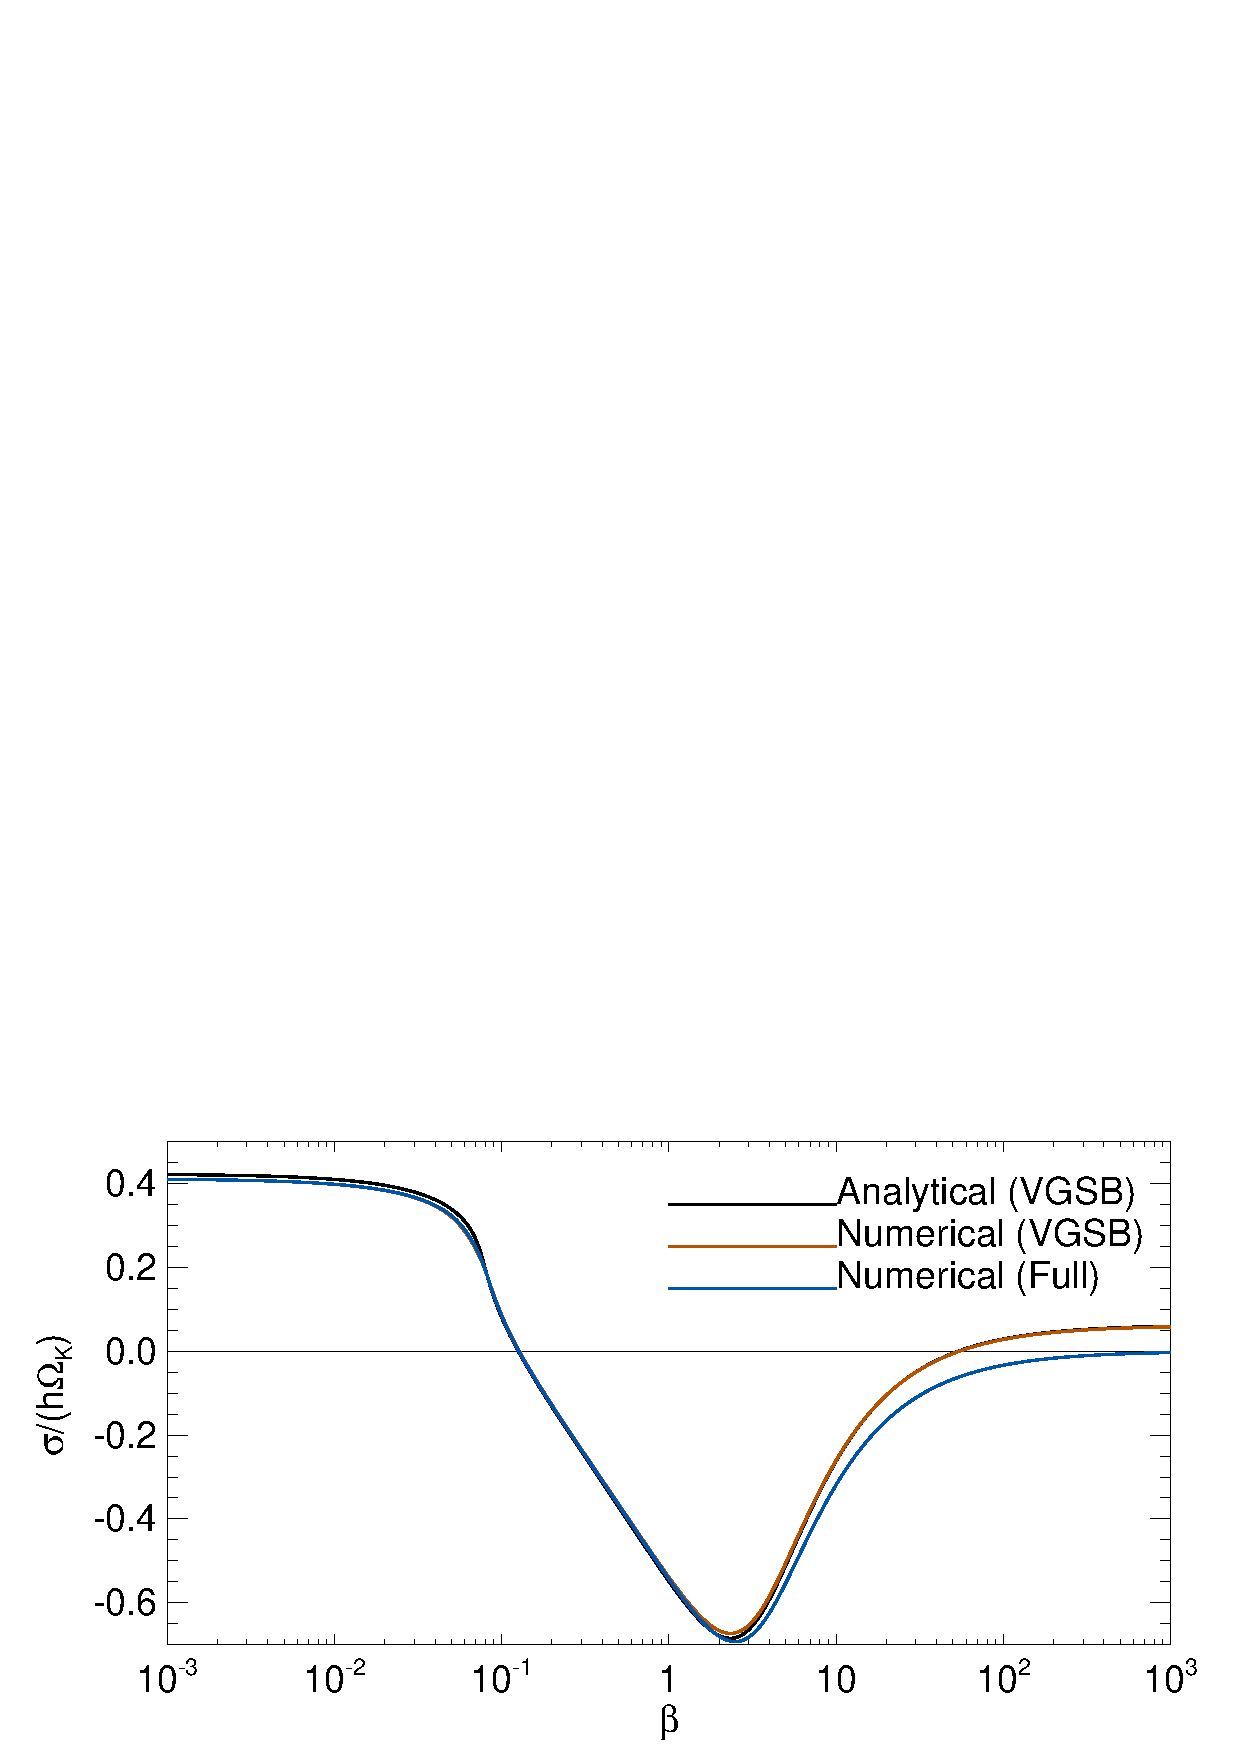
\includegraphics[width=\linewidth,clip=true,trim=0cm 0.0cm 0cm
  0cm]{figures/gcorr_compare} 
  \caption{Growth rate of the fundamental VSI mode as a function of
    the thermal relaxation time $\beta$. The `Analytical (VGSB)' curve
    is calculated from the dispersion relation Eq. \ref{relax_disp};
    the `Numerical (VGSB)' curve is obtained by numerically solving
    Eq. \ref{lin_mass}---\ref{lin_energy} with $\hat{g}_c=0$
    (which defines the linear VGSB equations); and the `Numerical
    (Full)' curve is obtained by numerically solving
    Eq. \ref{lin_mass}---\ref{lin_energy}  with $\hat{g}_c=1$, which
    accounts for the radial disk structure.  
% computed from the linear VGSB equations used in
%     the main text (dotted) and that including additional global
%     radial gradient terms in
%     Eq. \ref{gcorr_terms1}---\ref{gcorr_terms3} (solid). 
    The disk parameters are $\Gamma=1.011$,
    $\gamma=1.4$ and $(p,q,\epsilon)=(-1.5,-1,0.05)$. The perturbation
    wavenumber is $\khat=30$. 
    \label{gcorr_compare}}  
\end{figure}

Fig. \ref{gcorr_compare} shows that provided we consider $\beta\ll1$,
then the VGSB framework is an adequate approximation. It is
interesting to note that there is a thermal relaxation timescale that
maximizes the mode decay rate. Here, it is $\beta\simeq2$ or about
$0.3$ orbital periods. This is, in fact, consistent with Fig. 12 of
\cite{nelson13}.  




%nevertheless we have calculated
%plot growth rate v.s. bcool 
















\section{Full governing equation for vertically isothermal disks}\label{adia_improve}
% \section{Improving the nearly-Keplerian approximation for adiabatic
%   disks}\label{adia_improve}
In \S\ref{approx_gov} we made the replacement $D\to\Omega_k^2$ before
eliminating variables to obtain a single equation for $\delta v_z$,
Eq. \ref{vertiso_gov}.  This procedure ignores the vertical dependence of
$D=\kappa^2(z) - \sigma^2$. We show here that this has no significant
consequence for thin disks. 

In the global disk with $\Gamma=1$ we have
\begin{align}\label{dkappa2}
  \frac{\p\kappa^2}{\p z} = 4 \frac{\p\Omega^2}{\p z} + r\frac{\p}{\p
    r}\frac{\p\Omega^2}{\p z} = -
  \frac{\p\ln\rho}{\p z}\frac{qc_s^2}{r^2} \left(2 + q +
    \frac{z^2/r^2-2}{z^2/r^2+1}\right). 
\end{align}
For the local problem we may then write
\begin{align}
  \frac{dD}{dz}  = - \frac{d\ln\rho}{dz}\frac{qc_s^2}{r^2}F(z;q),
\end{align}
where the function $F$ corresponds to the bracket in
Eq. \ref{dkappa2}. This function varies from $F=q$ at $z=0$ to $F\to
3+q$ as $|z|\to\infty$, i.e. its magnitude is of order unity. 

 Eliminating $W$ and $Q$ from Eq. \ref{ode_w}---\ref{ode_Q} and
 Eq. \ref{lin_vz} for vertically isothermal disks, retaining the
 vertical dependence of $D$ and including thermal relaxation, we
 obtain 
\begin{align}
  0 =& \frac{d^2\delta v_z}{dz^2} + \left[1 + \frac{\ii k_x c_s^2
      q}{Dr} - \frac{k_x^2c_s^2}{\left(k_x^2c_s^2 + \chi
        D\right)}\frac{qc_s^2F}{Dr^2}\right]\frac{d\ln\rho}{dz}\frac{d\delta
    v_z}{dz} \notag\\
  &+ \left\{\sigma^2\left(\frac{k_x^2}{D} +
      \frac{\chi}{c_s^2}\right) + \left(\chi + \frac{\ii k_x c_s^2
        q}{Dr}\right)\frac{d^2\ln\rho}{dz^2} -
    \frac{c_s^2}{D}\left(\frac{d\ln\rho}{dz}\right)^2\left(k_x^2 -
      \frac{\ii k_x q}{r}\right)
   \left[\left(1-\chi\right) +
     \frac{\chi}{\left(k_x^2c_s^2 + \chi D\right)}\frac{qc_s^2 F}{r^2}\right] 
   \right\}\delta v_z,
\end{align}
where we recall $\chi = \left(1-\ii\sigma t_c\right)/\left(1-\ii\sigma
t_c \gamma\right)$. Making the low-frequency approximation with the
replacement $D\to \Omega_k^2$ gives, in terms of dimensionless
variables,
\begin{align}
   &\delta v_z ^{\prime\prime} + \left[1 + \ii\epsilon q\hat{k} -
    \frac{ \hat{k}^2}{
      \left(\hat{k}^2+\chi\right)}q \epsilon^2F\right]\ln\rho^{\prime}\delta v_z^\prime +
  \left\{\left(\chi + \ii \epsilon q
      \hat{k}\right)\ln\rho^{\prime\prime} - \ln\rho^{\prime
      2}\left(\khat^2 -
      \ii\epsilon
      q\hat{k}\right)\left[1 - \chi +
      \frac{\chi}{\left(\hat{k}^2+\chi\right)}q\epsilon^2F\right]\right\}\delta v_z \notag\\&=
  -\hat{\sigma}^2\left(\hat{k}^2+\chi\right)\delta v_z\label{adia_diso3}.
\end{align}   
Eq. \ref{adia_diso3} differs from Eq. \ref{vertiso_gov_nondim} by terms
proportional to $\epsilon^2$. For a thin disk, $\epsilon\ll1$, so
neglecting these terms has no qualitative effect on the discussion in
\S\ref{analytic_adia} and \S\ref{analytic_relax}.  This issue does not
arise for isothermal perturbations discussed in \S\ref{iso_discuss}
since in that case we work with a governing equation for $W$ instead. 

% \section{Alternative inference of instability in the presence of weak
%   vertical shear}\label{pert_theory}
% We can also investigate the destabilizing effect of vertical shear
% without explicitly solving the full governing equation,
% Eq. \ref{iso_ode3}. We first
% consider a system with $q\equiv0$, for which the eigenfunctions are
% Hermite polynomials and the real eigenfrequencies are known. We then
% perturb this system by introducing a weak vertical shear ($|q|\ll1$)
% and linearize the governing equation. This procedure is
% \begin{align}   
%   q \to 0 + \delta q,\quad
%   W \to \He_n + \delta W,\quad
%   \hat{\sigma} \to \hat{\sigma} + \delta\hat{\sigma}. 
% \end{align}
% %where for this exercise we restore $\sigma$ as the eigenfrequency. 

% Linearizing the integral relation Eq. \ref{integral_relation1} in the
% thin-disk limit, and taking the
% imaginary part, we have
% \begin{align}
%   2\hat{\sigma}\imag(\delta\hat{\sigma})
%   \left(1+\hat{k}^2\right) \int_{-\infty}^{\infty} w(\zhat)
%   \He_n^2(\hat{z}) d\hat{z}
%   = \delta q \epsilon \hat{k} 
%   \int_{-\infty}^{\infty}
%   w(\zhat)\hat{z}\He_n(\hat{z})\He_n^\prime(\zhat) d\hat{z}
% \end{align}
% Recognizing $\hat{z} = \He_1(\hat{z})$ and using $\He_n^\prime = n
% \He_{n-1}$ we have
%  \begin{align}
%    2\hat{\sigma}\imag(\delta\hat{\sigma})
%    \left(1+\hat{k}^2\right) \int_{-\infty}^{\infty} w(\zhat)
%    \He_n^2(\hat{z}) d\hat{z}
%    =\delta q \epsilon \hat{k} 
%    \int_{-\infty}^{\infty}
%    w(\zhat)\He_1(\hat{z})\He_n(\hat{z})n\He_{n-1}(\hat{z})d\hat{z}. 
%  \end{align}

% Finally, we evaluate the integrals using the results
% \begin{align}
%   \int_{-\infty}^{\infty}
%   w(\xi) \He_k(\xi)\He_l(\xi) d\xi = \sqrt{2\pi}k!\delta_{kl} \quad
% % \end{align}
% \text{and} \quad
% % \begin{align}
%   \int_{-\infty}^{\infty}
%   w(\xi) \He_m(\xi)\He_k(\xi)\He_l(\xi) d\xi =
%   \frac{\sqrt{2\pi}m!k!l!}{(j-m)!(j-k)!(j-l)!}, 
% \end{align}
% where $j = (m+k+l)/2$. We then obtain
%  \begin{align}
%    2\hat{\sigma}\imag(\delta\hat{\sigma})
%   \left(1+\hat{k}^2\right) = \delta q \epsilon \hat{k} n.
%  \end{align}
% Inserting the original eigenfrequency $\hat{\sigma} = \pm
% \sqrt{n}(1+\hat{k}^2)^{-1/2}$ gives
% \begin{align}
%   \imag(\delta\hat{\sigma})= \pm \frac{1}{2}\delta q \epsilon
%   \sqrt{n} \frac{\hat{k}}{\sqrt{1+\hat{k}^2}}. 
% \end{align}
% This result agrees with Eq. \ref{simple_growth} in the limit
% $|q|\to0$. 
% %for $n=1$, since the
% %function $\He_1$ solves the governing equation exactly. 
% For $\hat{k}\gg 1$ we have
% \begin{align}
%   \imag(\delta\hat{\sigma})\simeq \pm \frac{1}{2}\delta q \epsilon
%   \sqrt{n} \sgn{\hat{k}}. 
% \end{align}




% Differentiating Eq. \ref{adia_iso1} properly gives
% \begin{align}
%   \left(D + \gamma k_x^2 c_s^2\right)\frac{d\Delta}{dz}=& D
%   \frac{d^2\delta v_z}{dz^2} + k_x^2c_s^2\left[\frac{\gamma}{\left(D + \gamma k_x^2 c_s^2\right)}\frac{dD}{dz} + \ii
%     \frac{d\ln\rho}{dz}\left(\ii +
%       \frac{q}{k_xr}\right)\right]\frac{d\delta v_z}{dz}\notag\\
%   &+ \ii k_x^2 c_s^2 \left(\ii +
%       \frac{q}{k_xr}\right)\left[\frac{d^2\ln\rho}{dz^2} -
%       \frac{1}{\left(D + \gamma
%           k_x^2c_s^2\right)}\frac{dD}{dz}\frac{d\ln\rho}{dz}\right]\delta
%     v_z. \label{adia_diso1}
% \end{align}
% The terms that were ignored in deriving Eq. \ref{adia_iso3} are those
% proportional to $dD/dz$ in Eq. \ref{adia_diso1}. Now, in the global
% disk with $\Gamma=1$ we have
% \begin{align}\label{dkappa2}
%   \frac{\p\kappa^2}{\p z} = 4 \frac{\p\Omega^2}{\p z} + r\frac{\p}{\p
%     r}\frac{\p\Omega^2}{\p z} = -
%   \frac{\p\ln\rho}{\p z}\frac{qc_s^2}{r^2} \left(2 + q +
%     \frac{z^2/r^2-2}{z^2/r^2+1}\right). 
% \end{align}
% For the local problem we may then write
% \begin{align}
%   \frac{dD}{dz}  = - \frac{d\ln\rho}{dz}\frac{qc_s^2}{r^2}F(z;q),
% \end{align}
% where the function $F$ corresponds to the bracket in
% Eq. \ref{dkappa2}. This function varies from $F=q$ at $z=0$ to $F\to
% 3+q$ as $|z|\to\infty$, i.e. its magnitude is of order unity. 
% % We estimate the
% % importance of these terms by noting that 
% % \begin{align}
% %   \frac{dD}{dz}\equiv \frac{d\kappa^2}{dz} \simeq \frac{d\Omega^2}{dz}
% %   = - \frac{d\ln\rho}{dz}\frac{qc_s^2}{r^2},
% % \end{align}
% % for thin disks. 
% Eq. \ref{adia_diso1} becomes
% \begin{align}
% \left(D + \gamma k_x^2 c_s^2\right)\frac{d\Delta}{dz}=& D
%   \frac{d^2\delta v_z}{dz^2} - k_x^2c_s^2\frac{d\ln\rho}{dz}\left[ 1 - 
%       \frac{\ii q}{k_xr}  +  \frac{\gamma q c_s^2F}{r^2\left(D +
%         \gamma k_x^2 c_s^2\right)}\right]\frac{d\delta
%     v_z}{dz}\notag\\ 
%   &- k_x^2 c_s^2 \left(1 - 
%       \frac{\ii q}{k_xr}\right)\left[\frac{d^2\ln\rho}{dz^2} + 
%       \frac{qc_s^2F}{r^2\left(D + \gamma
%           k_x^2c_s^2\right)}\left(\frac{d\ln\rho}{dz}\right)^2\right]\delta
%     v_z. \label{adia_diso2}
% \end{align}
% Since $D\sim \Omega_k^2$ in the low-frequency limit, we 
% see from Eq. \ref{adia_diso2} that the neglected terms are
% $O(\epsilon^2)$. We can make this explicit by combining
% Eq. \ref{adia_diso1}---\ref{adia_diso2} and Eq. \ref{adia_iso2}, then
% set $D\to\Omega_k^2$. In terms of non-dimensional variables, the result
% is  
% \begin{align}
%    &\delta v_z ^{\prime\prime} + \left(1 + \ii\epsilon q\hat{k} -
%     \frac{\gamma q \epsilon^2\hat{k}^2F}{1+\gamma
%       \hat{k}^2}\right)\ln\rho^{\prime}\delta v_z^\prime +
%   \left[\left(\frac{1}{\gamma} + \ii \epsilon q
%       \hat{k}\right)\ln\rho^{\prime\prime} - \hat{k}^2\left(1 -
%       \frac{\ii\epsilon
%         q}{\hat{k}}\right)\left(\frac{\gamma-1}{\gamma} +
%       \frac{q\epsilon^2F}{1+\gamma\hat{k}^2}\right)\ln\rho^{\prime
%       2}\right]\delta v_z \notag\\&=
%   -\hat{\sigma}^2\left(\frac{1}{\gamma} + \hat{k}^2\right)\delta v_z\label{adia_diso3}.
% \end{align}   
% Eq. \ref{adia_diso3} differs from Eq. \ref{adia_iso3} by terms
% proportional to $\epsilon^2$. For a thin disk, $\epsilon\ll1$, so
% neglecting these terms has no qualitative effect on the discussion in
% \S\ref{analytic_adia}. 

\section{Coefficients for the dispersion relation for perturbations
with thermal relaxation}\label{relax_coeff}
The coefficients of the dispersion relation Eq. \ref{relax_disp} is
given by:
\begin{align}
  &c_0 = M(M+1)\widetilde{A}^2,\\
  &c_1 = \ii\beta\left\{\left(1-\gamma\right)\left[1 +
      \khat^2\left(1+2M\right)^2 - 4 \ii\epsilon q\khat M (M+1)\right] 
    - 2\widetilde{A}^2\gamma M (M+1)\right\},\\
  &c_2 = \left(\khat^2 + 1\right)\widetilde{A} + \beta^2\left\{(1-\gamma)\left[1
      + \gamma \khat^2(1+2M)^2 - 4\ii\epsilon q \khat \gamma M(M+1)
    \right]
    -\gamma^2 \widetilde{A}^2 M(M+1)
  \right\},\\
  &c_3 = \beta\left\{\epsilon q \khat + \gamma \left[\ii + \epsilon q
      k \left(1+2\khat^2\right)\right] - 3\ii - 2\ii
    \khat^2\right\},\\
  &c_4 =
  \beta^2\left(1+\gamma\khat^2\right)\left[\gamma\left(1-\ii\epsilon q
    \khat\right)-2\right] - \left(1+\khat^2\right)^2,\\
&c_5 = 2\ii\beta\left(1+\khat^2\right)\left(1+\gamma\khat^2\right),\\
&c_6 = \beta^2\left(1+\gamma\khat^2\right)^2.
\end{align}

\section{Fiducial model for a protoplanetary disk}\label{mmsn}
For results application in \S\ref{application} we use the disk model
described in \cite{chiang10}. This disk model orbits a Solar-mass star and 
has the surface density distribution
\begin{align}\label{mmsn_sigma}
  \Sigma = 2200
  \hat{\Sigma}\left(\frac{r}{\mathrm{AU}}\right)^{-3/2}\mathrm{g}\,\mathrm{cm}^{-2},  
\end{align}
and the temperature profile
\begin{align}\label{mmsn_temp}
  T = 120\hat{T}\left(\frac{r}{\mathrm{AU}}\right)^{-3/7} \mathrm{K},
\end{align}
which implies $q=-3/7$. In the above expressions, $\hat{\Sigma}$ and
$\hat{T}$ are dimensionless coefficients used to scale the model
relative to the MMSN. Their nomial values are unity. By assuming a
vertically isothermal disk, we deduce the disk aspect-ratio 
\begin{align}\label{mmsn_epsilon}
  \epsilon =
  3.36\times10^{-2}\left(\frac{\hat{T}}{\mu}\right)^{1/2}\left(\frac{r}{\mathrm{AU}}\right)^{2/7}, 
\end{align}
and the mid-plane density distribution 
\begin{align}
%  \rho_0 = 2.7\times10^{-9}
%  \hat{\Sigma}\left(\frac{r}{\mathrm{AU}}\right)^{-39/14}\mathrm{g}\,\mathrm{cm}^{-3},  
\rho_0 = 1.7\times10^{-9}
  \hat{\Sigma}\left(\frac{\hat{T}}{\mu}\right)^{-1/2}\left(\frac{r}{\mathrm{AU}}\right)^{-39/14}\mathrm{g}\,\mathrm{cm}^{-3},
\end{align}
which implies $p=-39/14$. 
%0.033576258
In addition, we
use the opacity model {\bf(reference?)}
 \begin{align}
   \kappa_d &= 2 \hat{\kappa}_d \left(\frac{T}{100\mathrm{K}}\right)^2
   \mathrm{cm}^2\,\mathrm{g}
    =
   2.88\hat{\kappa}_d\hat{T}^2\left(\frac{r}{\mathrm{AU}}\right)^{-6/7}\mathrm{cm}^2\,\mathrm{g}^{-1},   
 \end{align}
where the second equality follows from the model temperature profile
above, and $\hat{\kappa}_d$ has similar meaning as $\hat{\Sigma}$ and
$\hat{T}$. 


\bibliographystyle{apj}
\bibliography{ref}


\end{document}

